
% Første frame
\blueheader
\begin{frame}{2D: Ideen som forbinder integralet med den deriverte}
\begin{columns}[onlytextwidth]
  \begin{column}{0.45\textwidth}
    La \(A(x)\) være arealet mellom grafen til \(f\)  og x-aksen fra \(0\) til \(x\):
    \[
    A(x)=\int_{0}^{x} f(t)\,dt.
    \]

    For en liten økning \(\Delta x\) er arealet fra \(x\) til \(x+\Delta x\) omtrent lik $ f(x)\cdot\Delta x$
    \begin{align*}
      A(x+\Delta x)-A(x) &\approx f(x)\,\Delta x\\[0.8em]
      \frac{A(x+\Delta x)-A(x)}{\Delta x} &\approx f(x)\\[0.8em]
      A'(x) &\approx f(x)
    \end{align*}
  \end{column}
  \begin{column}{0.55\textwidth}
    \centering
    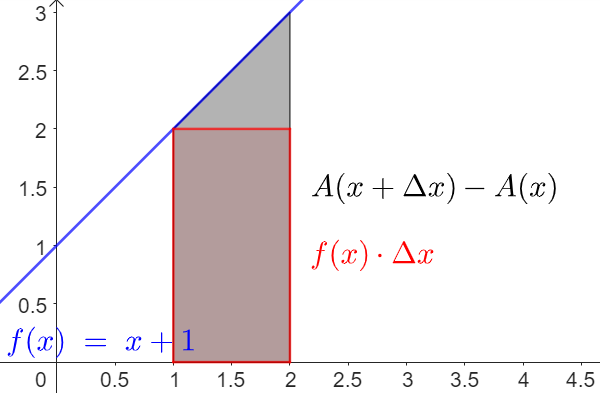
\includegraphics[width=\linewidth]{R2-K2A-4.png}
  \end{column}
\end{columns}
\end{frame}

% Andre frame
\greenheader
\begin{frame}{2D: Sammenhengen mellom posisjon og fart}
\begin{columns}[T,onlytextwidth]
   \begin{column}{0.45\textwidth}
    \begin{align*}
      s(t+\Delta t)-s(t) &\approx v(t)\,\Delta t\\[0.8em]
      \frac{s(t+\Delta t)-s(t)}{\Delta t} &\approx v(t)\\[0.8em]
      s'(t) &\approx v(t)
    \end{align*}
  \end{column}
   \begin{column}{0.55\textwidth}
    \centering
    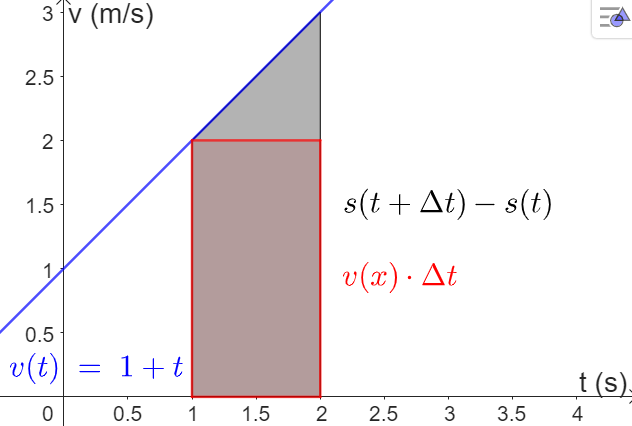
\includegraphics[width=\linewidth]{R2-K2A-5.png}
  \end{column}
\end{columns}
\end{frame}

